% Slides do trabalho final — compilar a partir da raiz do repositório:
%   pdflatex slides.tex
% Cada pessoa edita os seus slides (marcados com % Pessoa N).
% Os textos de H1 e H3 são um rascunho a partir dos resultados: Pessoas 1 e 3, revisem.
\documentclass[aspectratio=169,11pt]{beamer}

\usepackage[utf8]{inputenc}
\usepackage[T1]{fontenc}
\usepackage[brazilian]{babel}
\usepackage{booktabs}
\usepackage{graphicx}
\usepackage{xcolor}

\usepackage{tikz}

% ---------------------------------------------------------------------
% Visual próprio (sem pacotes externos de tema)
% ---------------------------------------------------------------------
\definecolor{escuro}{HTML}{1D2D44}   % azul-marinho
\definecolor{destaque}{HTML}{2A9D8F} % verde-azulado
\definecolor{alerta}{HTML}{E76F51}   % coral
\definecolor{suave}{HTML}{F4F6F8}    % cinza bem claro
\definecolor{cinza}{HTML}{8D99AE}

\usefonttheme{professionalfonts}
\setbeamertemplate{navigation symbols}{}
\setbeamercolor{normal text}{fg=escuro}
\setbeamercolor{structure}{fg=destaque}
\setbeamercolor{alerted text}{fg=alerta}
\setbeamercolor{frametitle}{fg=escuro}
\setbeamerfont{frametitle}{size=\Large,series=\bfseries}

% Título do slide: texto à esquerda + filete colorido
\setbeamertemplate{frametitle}{%
  \vspace*{0.6em}%
  \begin{beamercolorbox}[wd=\paperwidth,leftskip=1.2em]{frametitle}%
    \usebeamerfont{frametitle}\insertframetitle
  \end{beamercolorbox}%
  \vspace*{0.15em}%
  \hspace*{1.2em}{\color{destaque}\rule{2.5em}{2.5pt}}%
}

% Rodapé: barra de progresso + título curto + número
\setbeamertemplate{footline}{%
  \ifnum\insertframenumber>1
  \begin{tikzpicture}[remember picture,overlay]
    \fill[suave] (current page.south west) rectangle ([yshift=3pt]current page.south east);
    \fill[destaque] (current page.south west) rectangle
      ([yshift=3pt,xshift={\insertframenumber/\inserttotalframenumber*\paperwidth}]current page.south west);
  \end{tikzpicture}%
  \hspace*{1.2em}{\color{cinza}\tiny\insertshorttitle}\hfill
  {\color{cinza}\tiny\insertframenumber\,/\,\inserttotalframenumber}\hspace*{1.2em}%
  \vspace*{0.7em}%
  \fi
}

% Marcadores de lista
\setbeamertemplate{itemize item}{\color{destaque}\raisebox{0.15ex}{\rule{0.45em}{0.45em}}}
\setbeamertemplate{itemize subitem}{\color{cinza}\textbullet}
\setbeamerfont{description item}{series=\bfseries}

% Blocos: título colorido, corpo claro
\setbeamertemplate{blocks}[default]
\setbeamercolor{block title}{fg=white,bg=destaque}
\setbeamercolor{block body}{fg=escuro,bg=suave}
\setbeamerfont{block title}{series=\bfseries,size=\normalsize}

% Capa
\setbeamertemplate{title page}{%
  \begin{tikzpicture}[remember picture,overlay]
    \fill[escuro] (current page.south west) rectangle (current page.north east);
    \fill[destaque] ([xshift=1.2cm,yshift=-3.1cm]current page.north west) rectangle ++(2.2cm,0.12cm);
    \node[anchor=north west,text width=0.85\paperwidth,align=left,text=white]
      at ([xshift=1.2cm,yshift=-3.5cm]current page.north west)
      {{\LARGE\bfseries\inserttitle}\\[0.6em]{\large\color{destaque!60!white}\insertsubtitle}};
    \node[anchor=south west,text width=0.85\paperwidth,align=left,text=white!85!escuro]
      at ([xshift=1.2cm,yshift=1.0cm]current page.south west)
      {{\small\insertauthor}\\[0.3em]{\footnotesize\color{cinza}\insertinstitute\ \textbullet\ \insertdate}};
  \end{tikzpicture}%
}

% Slide de abertura de cada seção
\AtBeginSection[]{%
  \begin{frame}[plain,noframenumbering]
    \begin{tikzpicture}[remember picture,overlay]
      \fill[escuro] (current page.south west) rectangle (current page.north east);
      \node[anchor=west,text=destaque,font=\fontsize{60}{60}\selectfont\bfseries]
        at ([xshift=1.2cm]current page.west) {\thesection};
      \node[anchor=west,text=white,font=\huge\bfseries]
        at ([xshift=3.6cm]current page.west) {\insertsectionhead};
    \end{tikzpicture}
  \end{frame}
}

\newcommand{\pendente}[1]{\textcolor{alerta}{[#1]}}
% Caixa de destaque para números grandes
\newcommand{\numero}[2]{%
  \begin{minipage}[t]{0.3\textwidth}\centering
    {\color{destaque}\fontsize{26}{28}\selectfont\bfseries #1}\\[0.3em]
    {\small #2}
  \end{minipage}}

\title[Representação dos dados e classificadores]{O impacto da representação dos dados\\
no desempenho de classificadores}
\subtitle{Um estudo com a base \emph{Dry Bean}}
\author[Grupo]{Arthur Andrade \textbullet\ Fernanda Cruz \textbullet\ Isabelle Gonçalves \textbullet\ Thiago Fraga \textbullet\ Wagner Duarte}
\institute[UFMG]{Introdução ao Reconhecimento de Padrões \textbullet\ UFMG}
\date{Novembro de 2026}

\begin{document}

\begin{frame}[plain]
  \titlepage
\end{frame}

%% ====================================================================
%% Pessoa 4: base, hipóteses e protocolo
%% ====================================================================
\section{Base e protocolo}

\begin{frame}{A base \emph{Dry Bean}}
  % Pessoa 4
  \vspace{0.5em}
  \centering
  \numero{13.611}{grãos de feijão}\hfill
  \numero{16}{atributos de tamanho e forma}\hfill
  \numero{7}{variedades (classes)}

  \vspace{1.2em}
  \raggedright
  \begin{columns}[T]
    \begin{column}{0.48\textwidth}
      \begin{itemize}
        \item Atributos extraídos de imagens, sem valores faltantes
        \item Classes desbalanceadas: Dermason 26\,\% \dots{} Bombay 3,8\,\%
      \end{itemize}
    \end{column}
    \begin{column}{0.48\textwidth}
      \begin{itemize}
        \item Escalas muito diferentes (\texttt{Area} $\sim 10^4$, fatores de forma $<1$)
        \item Atributos fortemente correlacionados
      \end{itemize}
    \end{column}
  \end{columns}
  \vfill
  \pendente{Opcional: figura da análise exploratória (classes ou correlação)}
\end{frame}

\begin{frame}{Hipóteses}
  % Pessoa 4
  \begin{description}[H1]
    \item[H1] A padronização ajuda muito o KNN e o SVM, mas quase não muda o Naive Bayes.
    \item[H2] Remover atributos redundantes ajuda o Naive Bayes, mas quase não muda o KNN e o SVM.
    \item[H3] Com o mesmo número de dimensões, o PCA tem desempenho melhor do que a
      remoção de atributos correlacionados.
  \end{description}
  \vfill
  Classificadores: KNN ($k=5$), Naive Bayes gaussiano e SVM (RBF), com hiperparâmetros padrão.
\end{frame}

\begin{frame}{Protocolo experimental}
  % Pessoa 4
  \begin{itemize}
    \item Validação cruzada estratificada: 5 \emph{folds} $\times$ 3 repetições
      (15 execuções), \texttt{random\_state}$=42$
    \item Transformações ajustadas só no treino de cada \emph{fold}
      (\texttt{Pipeline} do \texttt{scikit-learn}), sem vazamento
    \item Métrica principal: \textbf{F1-macro}, por causa do desbalanceamento
    \item Também: acurácia, tempo e matrizes de confusão
    \item Resultados como média $\pm$ desvio padrão
    \item Mesmas divisões para tudo: comparação pareada por \emph{fold}
      (teste $t$ corrigido de Nadeau e Bengio na H2 e na H3)
  \end{itemize}
\end{frame}

%% ====================================================================
%% Pessoa 1: H1
%% ====================================================================
\section{H1: escala dos atributos}

\begin{frame}{H1: impacto da escala dos atributos}
  % Pessoa 1
  \centering
  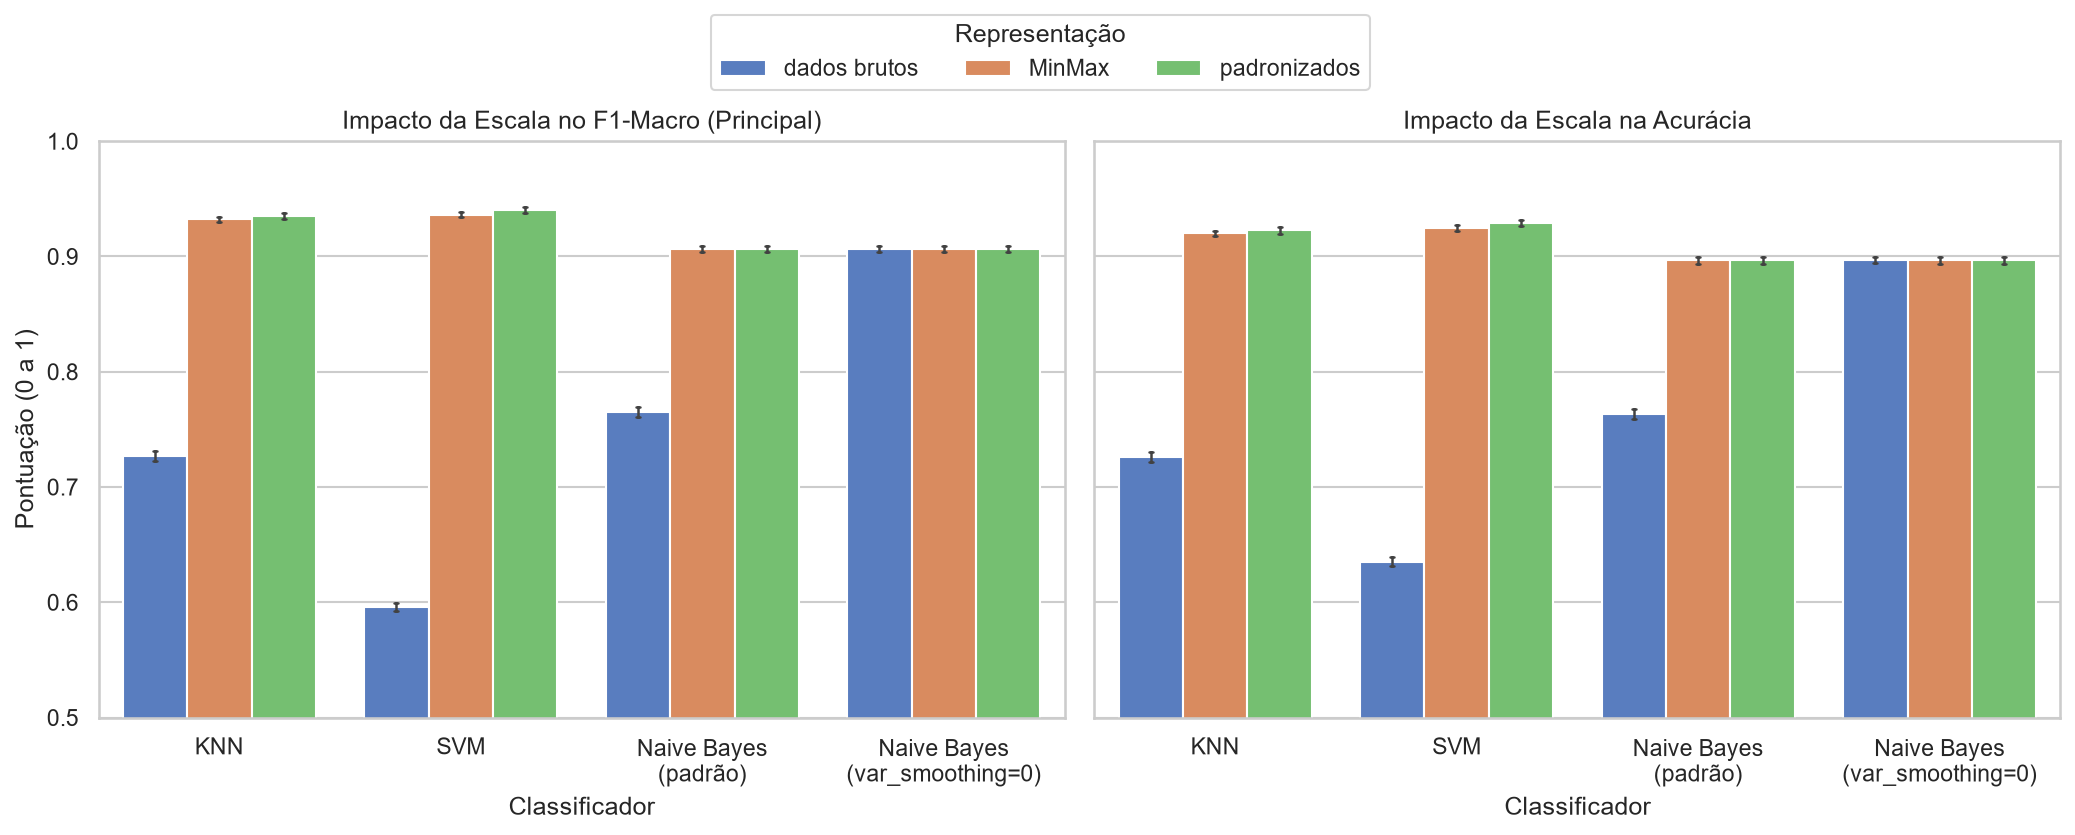
\includegraphics[width=\textwidth]{resultados/H1/h1_comparacao_metricas.png}
\end{frame}

\begin{frame}{H1: resultados e avaliação}
  % Pessoa 1
  \centering
  \numero{+20,8}{p.p.\ no KNN\\com padronização}\hfill
  \numero{+34,4}{p.p.\ no SVM\\(de pior a melhor)}\hfill
  \numero{0,0}{p.p.\ no Naive Bayes\\(\texttt{var\_smoothing=0})}

  \vspace{1em}
  \raggedright
  \begin{itemize}
    \item Nos dados brutos, atributos grandes (\texttt{Area}) dominam a distância e o núcleo RBF
    \item O ganho de +14,1 p.p.\ do Naive Bayes padrão é um \alert{artefato do \texttt{var\_smoothing}}
  \end{itemize}
  \begin{block}{Avaliação}
    H1 \textbf{confirmada} (isolado o artefato do \texttt{var\_smoothing}): KNN e SVM dependem da escala;
    o Naive Bayes é invariante a ela.
  \end{block}
\end{frame}

%% ====================================================================
%% Pessoa 2: H2
%% ====================================================================
\section{H2: atributos redundantes}

\begin{frame}{H2: remoção de atributos redundantes}
  % Pessoa 2
  \centering
  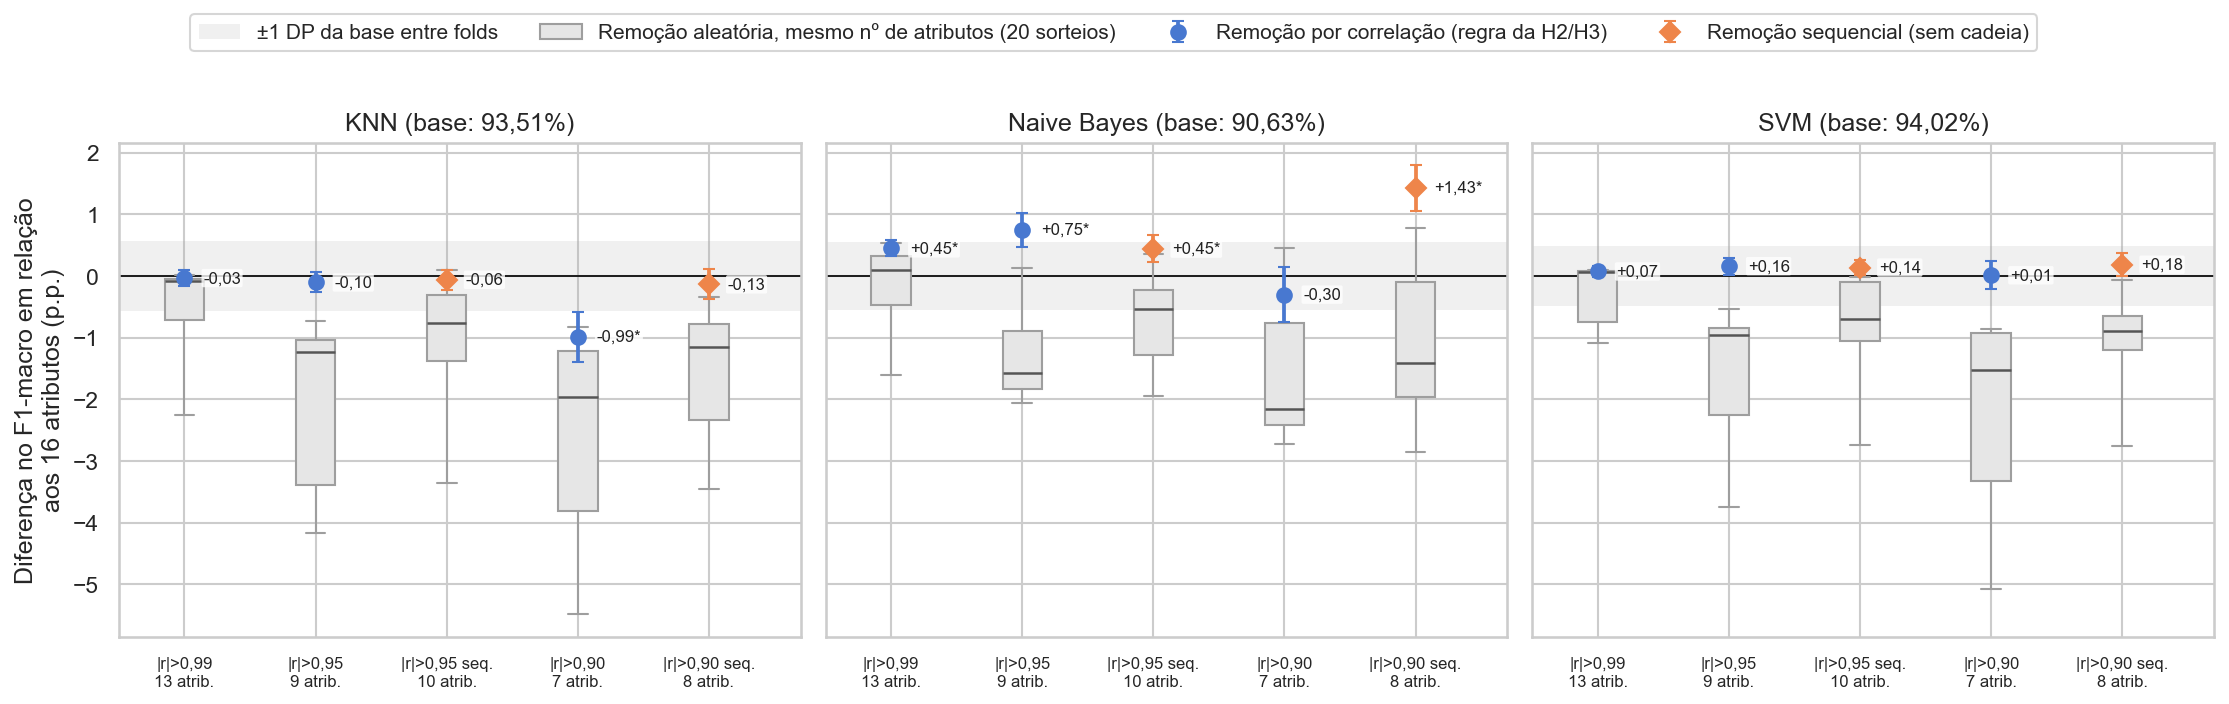
\includegraphics[width=\textwidth]{resultados/H2/h2_efeito_remocao.png}

  \small Diferença no F1-macro em relação aos 16 atributos padronizados, pareada por \emph{fold}
  (* $p<0{,}05$, teste $t$ corrigido).
\end{frame}

\begin{frame}{H2: resultados e avaliação}
  % Pessoa 2
  \centering
  \numero{+0,75}{p.p.\ no Naive Bayes\\($|r|>0{,}95$, 15/15 \emph{folds})}\hfill
  \numero{+1,43}{p.p.\ no Naive Bayes\\(sem remoção em cadeia)}\hfill
  \numero{$\leq$0,18}{p.p.\ no KNN e no SVM\\(sem significância)}

  \vspace{0.8em}
  \raggedright
  \begin{itemize}
    \item O Naive Bayes conta o tamanho 6$\times$ e abafa a forma: o ganho vem do par Barbunya/Cali
    \item Remoção aleatória do mesmo tamanho piora (em média, até 2,7 p.p.): a regra tira só redundância
    \item Em $|r|>0{,}90$ o KNN perde 0,99 p.p.: \texttt{ShapeFactor1} sai \alert{em cadeia}
  \end{itemize}
  \begin{block}{Avaliação}
    H2 \textbf{confirmada} em $|r|>0{,}99$ e $0{,}95$ e refutada em $0{,}90$, com efeito pequeno
    (da ordem do desvio entre \emph{folds}).
  \end{block}
\end{frame}

%% ====================================================================
%% Pessoa 3: H3
%% ====================================================================
\section{H3: PCA $\times$ remoção}

\begin{frame}{H3: PCA $\times$ remoção com o mesmo número de dimensões}
  % Pessoa 3
  \centering
  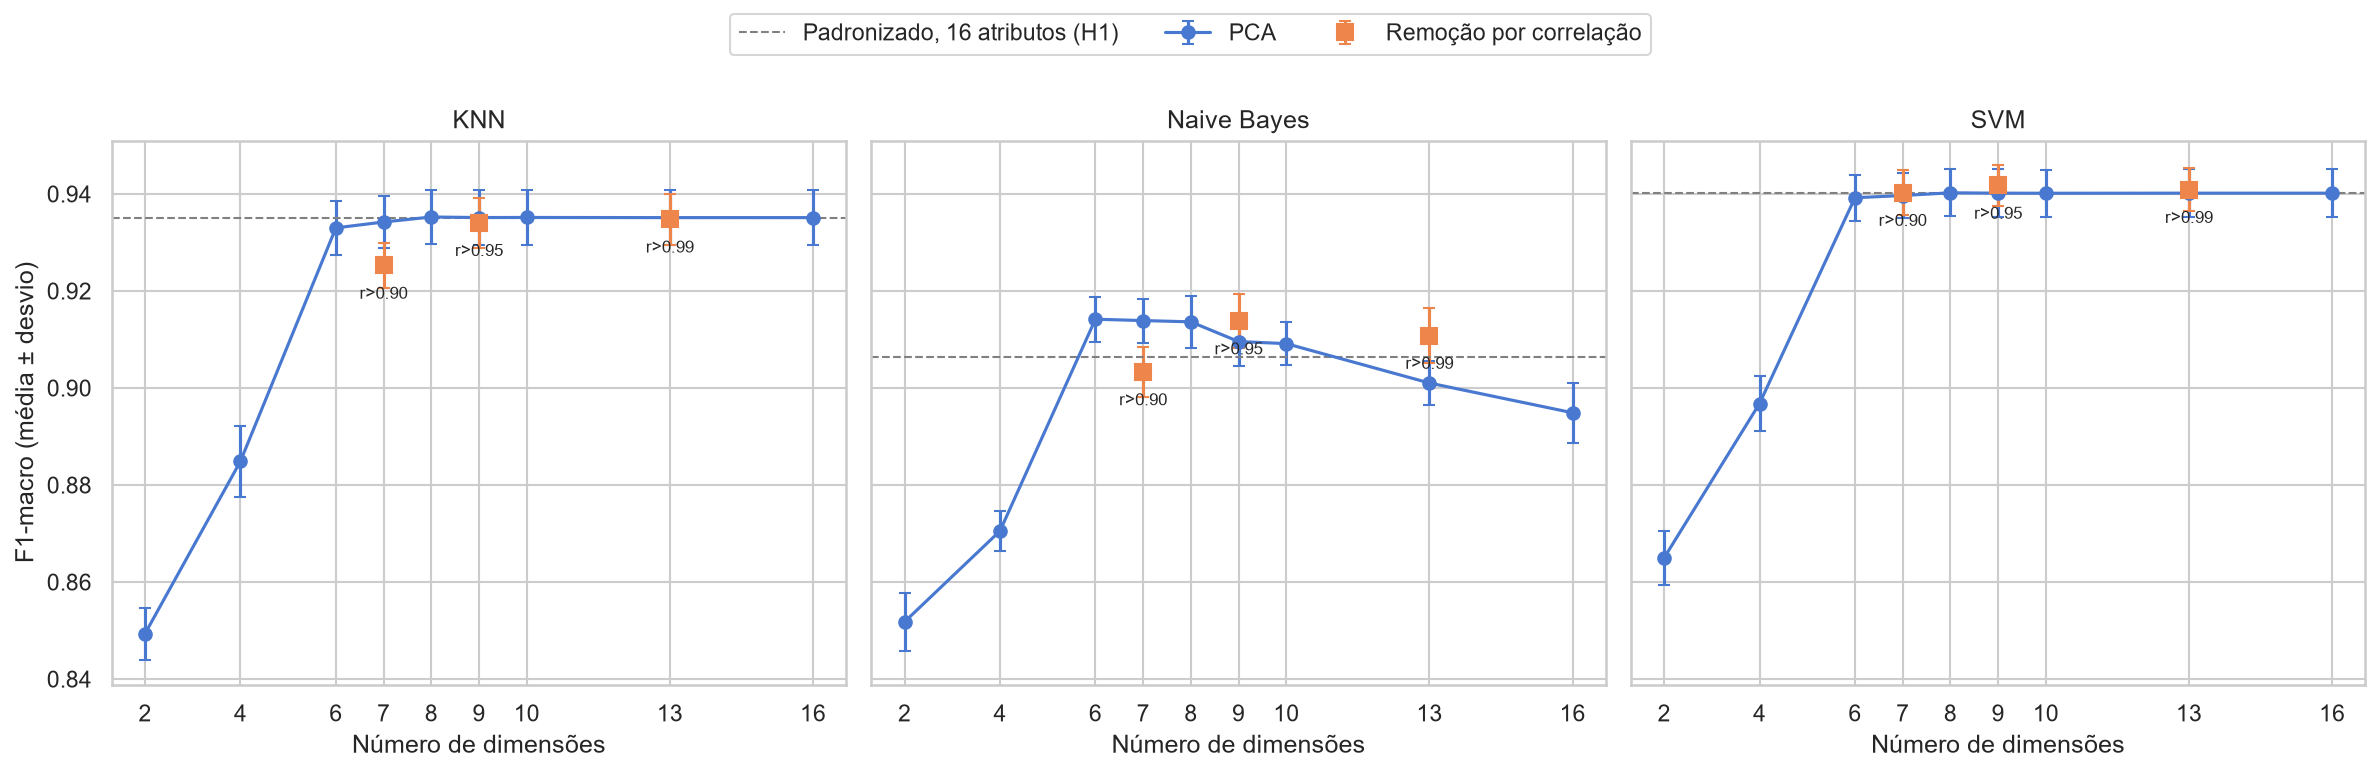
\includegraphics[width=\textwidth]{resultados/H3/h3_f1_por_dimensao.png}
\end{frame}

\begin{frame}{H3: resultados e avaliação}
  % Pessoa 3
  \centering\small
  \begin{tabular}{lccc}
    \toprule
    & \multicolumn{3}{c}{Diferença PCA $-$ remoção (p.p.)} \\
    \cmidrule(lr){2-4}
    \textbf{Classificador} & 7 dim.\ ($r>0{,}90$) & 9 dim.\ ($r>0{,}95$) & 13 dim.\ ($r>0{,}99$) \\
    \midrule
    KNN         & \textbf{+0,89} & +0,11 & +0,03 \\
    Naive Bayes & \textbf{+1,06} & $-$0,42 & $-$0,98 \\
    SVM         & $-$0,06 & $-$0,16 & $-$0,07 \\
    \bottomrule
  \end{tabular}

  \raggedright
  \begin{itemize}
    \item Com 7 dimensões, o PCA vence em 15/15 \emph{folds} no KNN e no NB ($t$ corrigido, $p<0{,}001$)
    \item Com menos remoção, a vantagem some ou se inverte (NB com 13 dim.: remoção melhor, $p<0{,}01$);
      no SVM tudo fica abaixo de 0,2 p.p.
  \end{itemize}
  \begin{block}{Avaliação}
    H3 \textbf{parcialmente confirmada}: o PCA só ajuda quando a remoção descarta atributos informativos
    (com 7 dimensões, \texttt{ShapeFactor1} sai \alert{em cadeia}; sem isso, a remoção empata ou vence).
  \end{block}
\end{frame}

%% ====================================================================
%% Pessoa 5: comparação geral e conclusão
%% ====================================================================
\section{Comparação e conclusão}

\begin{frame}{Comparação geral}
  % Pessoa 5 — figura gerada por codigos/comparacao_geral.py
  \begin{columns}[c]
    \begin{column}{0.62\textwidth}
      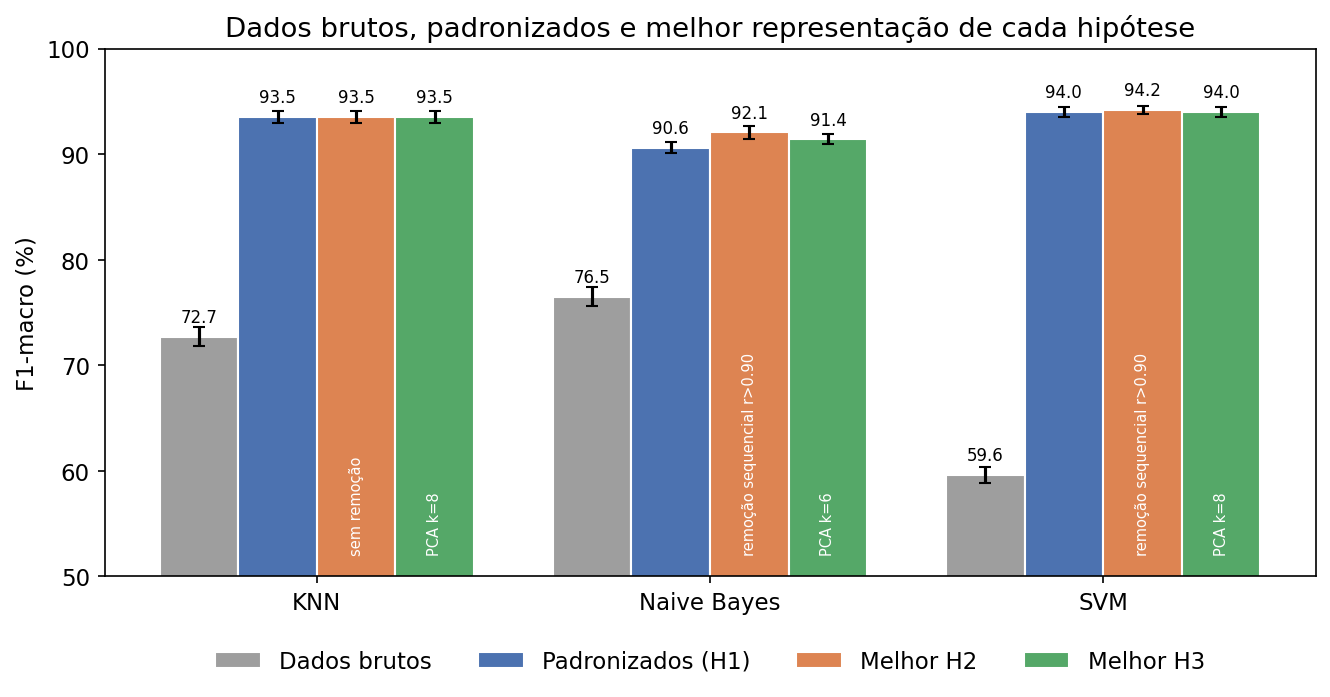
\includegraphics[width=\textwidth]{resultados/geral/geral_melhores_por_hipotese.png}
    \end{column}
    \begin{column}{0.36\textwidth}
      \small
      \begin{itemize}
        \item Escala: ganho de \textbf{21 a 34 p.p.}\ no KNN e no SVM
        \item Depois de padronizar, reduções que preservam a informação mudam \textbf{no máximo 1,4 p.p.}
          (com $k\leq4$, perda de 3,6 a 8,6 p.p.)
        \item Só o Naive Bayes ganha algo: +1,4 p.p.\ tirando redundância (H2), +0,8 p.p.\ com PCA (H3)
        \item Remoção aleatória piora: o ganho vem da \textbf{redundância}
        \item 6 componentes bastam: perda $\leq$ 0,25 p.p.
      \end{itemize}
    \end{column}
  \end{columns}
\end{frame}

\begin{frame}{Conclusão}
  % Pessoa 5
  \begin{itemize}
    \item \textbf{H1 confirmada} \quad \textbf{H2 confirmada} (0,99 e 0,95) \quad
      \textbf{H3 parcialmente confirmada}
    \item A \textbf{representação pesou mais que o classificador}:
      \begin{itemize}
        \item dados brutos: 17 p.p.\ entre o melhor e o pior (SVM em último)
        \item padronizados: menos de 3,5 p.p.\ entre os três (SVM em primeiro)
      \end{itemize}
    \item Depois da escala, o maior ganho é do Naive Bayes ao tirar \textbf{atributos repetidos}
      (+1,4 p.p.)
  \end{itemize}
  \vfill
  \begin{block}{Limitações}
    Hiperparâmetros padrão $\cdot$ uma única base $\cdot$ regra de remoção depende da ordem
    e remove em cadeia $\cdot$ diferenças $<1{,}5$ p.p.\ da ordem do desvio entre \emph{folds}
  \end{block}
\end{frame}

\begin{frame}[plain]
  \begin{tikzpicture}[remember picture,overlay]
    \fill[escuro] (current page.south west) rectangle (current page.north east);
    \node[text=white,font=\Huge\bfseries] at ([yshift=0.5cm]current page.center) {Obrigado!};
    \node[text=destaque,font=\large] at ([yshift=-0.6cm]current page.center) {Perguntas?};
  \end{tikzpicture}
\end{frame}

\end{document}
